\subsection{\textbf{Event Based Techniques}}
\label{sec:EventBased}

Much discussion has been aimed at the negative affect divergence in Monte Carlo codes has on  performance.
%
Given the inherently parallel nature of the algorithm, each particle being tracked independently, performance of Monte Carlo transport codes on the GPU should be incredible.
%
We often see the opposite and have seen throughout this section the different approaches and often marginal speedups that were attained.
%
One main concern with many of these studies was the affect divergence had on their algorithm.
%

%
In order to combat divergence, a old scheme was re-evaluated for use on GPU architectures.
%
Given some of the similarities between the classic vector machines of the 1980's/90's with modern GPU hardware, it is reasonable to consider some of those algorithms for use now.
%
One main approach that worked well on SIMD vector hardware, is the event-based approach.
%
In the event-based approach particles are processed in groups that are performing the same event.
%
There are multiple variations to this idea and a few of those are presented here.
%

\subsection*{\textbf{Vectorized Algorithm}}

%
Early event based algorithms were designed for vector machines and were called vectorized algorithms.
%
Martin describes a successful vectorized algorithm as well some variations in his paper~\cite{martin1989successful}.
%
The conventional Monte Carlo algorithm cannot be vectorized since treating many histories simultaneously would immediately fail after the first step of the simulation as each particle can undergo a different event.
%
In order to achieve vectorization the histories need to be split into events, which are similar and can be processed in a vectorized manner, i.e. the same set of instructions.
%
The basic event based iteration algorithm is descirbed in Algorithm~\ref{alg:basicEvent}.
%

%
\begin{algorithm}
\DontPrintSemicolon
\caption{The basic iteration event}
\label{alg:basicEvent}
\For{ event n = 0, 1, 2, ... }
{
	$\cdot$ Fetch $\Gamma^{n}$ \\
	$\cdot$ Preform free flight analysis:\\
	\Indp	$\cdot$ gather the cross section data and geometry data tabulated by particle,\\
		$\cdot$ $\Sigma \leftarrow$ S,\\
		$\cdot$ $\rho \leftarrow$ R;\\
		$\cdot$ using $\Sigma$, sample a vector of distances to collision, $d_{c}$\\
		$\cdot$ using $\rho$, determine vector of minimum distances to boundary, $d_{b}$\\
		$\cdot$ determine the minimum distances to the end of event,\\
		\Indp $d_{min}$ = min[$d_{c}, d_{b}$];\\
		\Indm $\cdot$ update the particle coordinates,\\
		\Indp $r^{n+1}$ = $r^{n} + \Omega^{n} \cdot r_{min}$\\
	\Indm $\cdot$ Perform collision analysis:\\
	\Indp $\cdot$ gather particle attributes,\\
	\Indp $\Omega \leftarrow \Gamma^{n}, E \leftarrow \Gamma^{n}$;\\
	\Indm $\cdot$ evaluate collision physics for new direction cosines and energies,\\
	\Indp $\Omega ' \leftarrow \Omega$, $E' \leftarrow  E$\\
	\Indm $\cdot$ scatter new particle attributes back into bank,\\
	\Indp $\Omega ' \leftarrow \Gamma^{n}$, $E' \leftarrow  \Gamma^{n}$\\
	\Indm \Indm $\cdot$ Perform the boundary analysis:\\
	\Indp $\cdot$ gather particle zone indices $Z$,\\
	\Indp $Z \leftarrow \Gamma^{n}$\\
	\Indm $\cdot$ determine new zone indices,\\
	\Indp $Z' \leftarrow Z:$\\
	\Indm $\cdot$ scatter new zone indices back into bank.\\
	\Indp $Z' \rightarrow \Gamma^{n}$\\
	\Indm \Indm $\cdot$ Update the particle bank,\\
	\Indp $\Gamma^{n} \Rightarrow \Gamma^{n+1}\ (with\ L_{n+1}\ particles )$ \\
	(e.g. compress out terminated particles).\\
	\Indm $\cdot$ If $L_{n+1} \neq 0, continue$\\
%	\State using \Sigma, sample a vector of distances to collision, $d_{c}$
%	\EndIndent
}
\end{algorithm}
%

In addition to the basic event based approach there are a few variations discussed in Martins paper that expand on this model.
%
One variation is the stack-driven approach.
%
In this approach the events are further divided into smaller computational tasks.
%
Instead of cycling through the tasks in a fixed order, the computation can move forward by selecting the event with the largest number of particles.
%
This involves a tradeoff of simplified control flow for maximizing the vector lengths of the computational components.
%

%
Vectorized versions of the Monte Carlo transport algorithms are all based on this original basic algorithm.
%
There are many variations but the principal differences all depend on the methods used for organizing and treating the vectors of particles.
%
There are variations using stack, tags, and tasks.
%
The major downside to the event based approach is that is requires a large change to pre-existing source code.
%

\subsection*{\textbf{Event Based for GPU}}

%
Event based methods used for the GPU follow similar design patterns as those that were developed for vector machines.
%
One prime example is the event based version developed by Bergmann for the code WARP~\cite{2014development}.
%
Figure~\ref{fig:innerLoopWARP} outlines the inner transport loop broken into its separate stages.
%
Figure~\ref{fig:outerLoopWARP} outlines the outer transport loop between neutron batches.
%

\begin{figure}
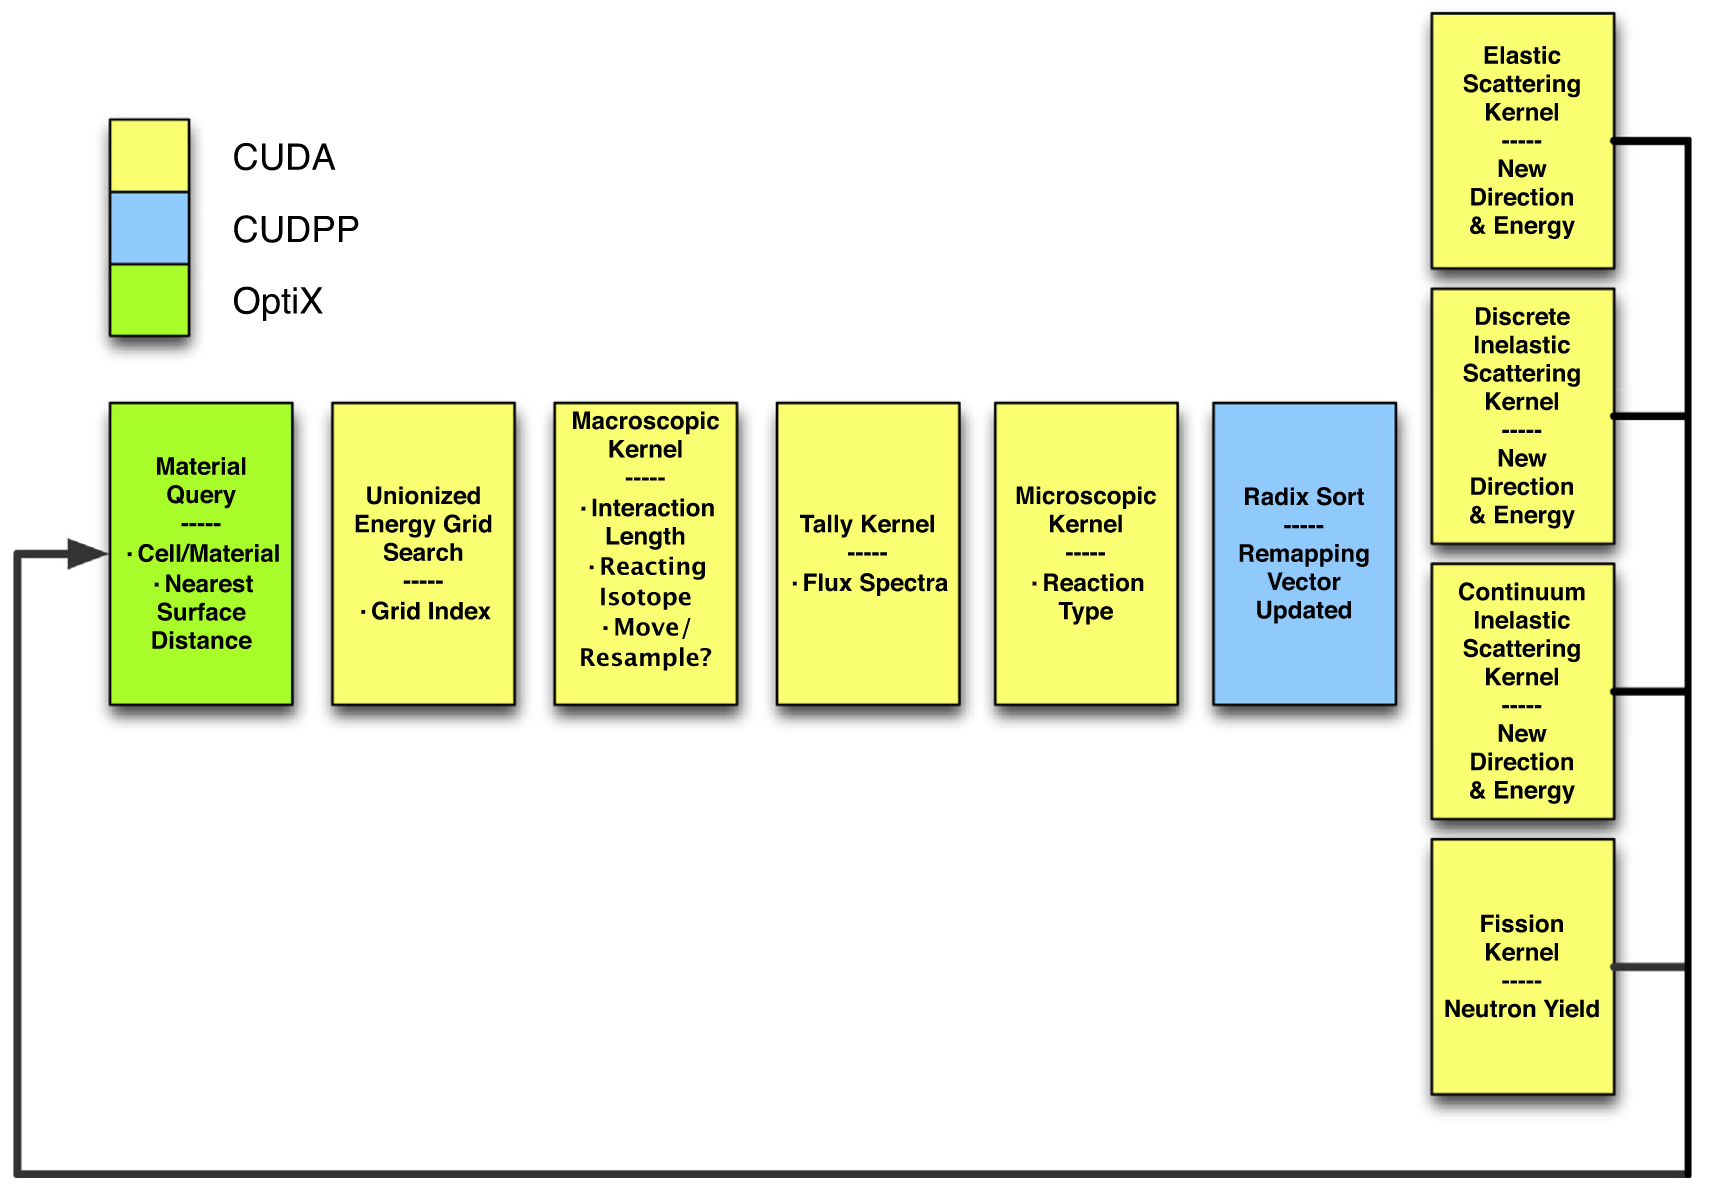
\includegraphics[width=0.49\textwidth]{InnerLoopWARP}
\caption{WAP inner tranport loop that is executed until all neutrons in a batch are completed~\cite{2014development}}
\label{fig:innerLoopWARP}
\end{figure}

\begin{figure}
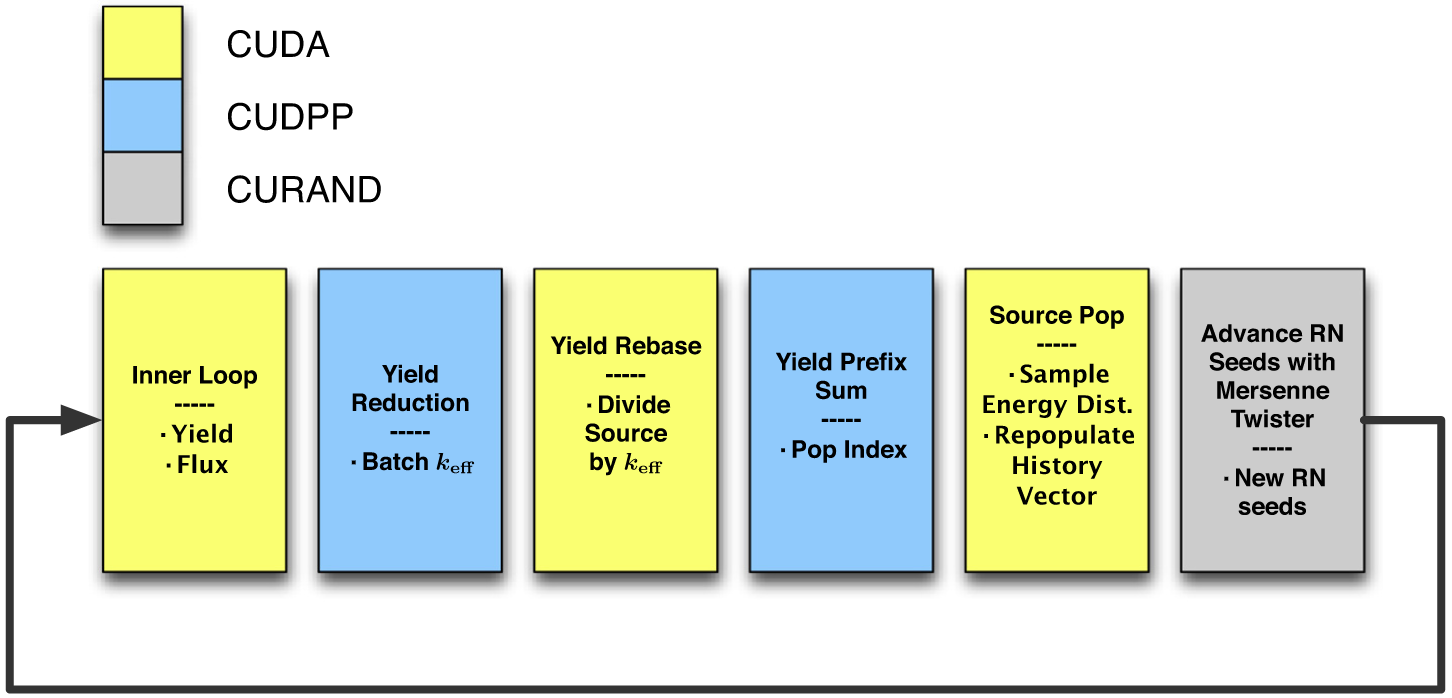
\includegraphics[width=0.49\textwidth]{OuterLoopWARP}
\caption{WAP inner tranport loop that is executed until all neutrons in a batch are completed~\cite{2014development}}
\label{fig:outerLoopWARP}
\end{figure}

Bergmann's event based Monte Carlo code WARP~\cite{2014development} utilizes a series of kernels that each solves one piece of the process.
%
Once each neutron knows which path it will go down -- i.e. scattering, fission, etc. -- each of those possible paths is launched in a separate kernel.
%
Unlike the basic vectorized approach or the stack based approach however, all of the events are launched at once using concurrent kernels due to CUDA streaming properties.
%
In this way, the main divergent part of the code is broken into relatively non-divergent kernels which are then launched simultaneously so as to continue to utilize the full hardware.

Not all attempts at vectorization, or implementing an event based algorithm for Monte Carlo transport codes has been successful.
%
Liu~\cite{liu2014comparative} describes an event-based approach that after being implemented produced a roughly ten times slower version then the history-based code.
%
This example shows how complicated the task of implementing an event-based algorithm can be, and that it is possible as well that not all Monte Carlo transport problems can be solved efficiently in an event-based fashion.
%
Liu attributed their slow down to the memory access latency due to the high amount of global memory transactions and showed that the cost of this in an event-based method did not outweigh the benefit of reducing thread divergence and increasing warp execution efficiency.





